\documentclass[a4paper,12pt]{article}
\usepackage[a4paper,left=3cm,right=3cm,top=3cm,bottom=3cm]{geometry}

\usepackage{endfloat}


\usepackage[utf8]{inputenc}
\usepackage[english]{babel}
\usepackage[babel]{csquotes}

\usepackage{amsmath}
\usepackage{amssymb}

\usepackage[colorlinks=true, allcolors=blue]{hyperref}
\usepackage[all]{hypcap}

\usepackage{graphicx}
\usepackage{subcaption}

\usepackage[style=authoryear, backend=biber]{biblatex}  
\bibliography{~/Zotero/Bibliothek.bib}

%opening
\title{Time will tell: Incorporating Attention Span into Diffusion Models}

\author{Malte Grönemann}

\begin{document}

\maketitle

\section{Introduction}

Scholars from various social science disciplines have been interested in diffusion processes: whether they considered the demand of new products by consumers, the spread of information within the public, the patterns of the transmission of contagious diseases, the emergence of new norms or movements in a society or changes in individual behaviours. But despite all their differences in specific applications, disciplines and research traditions, they typically share a common distinction in their conceptualisation: they can either spread from external sources or through human interaction. A household might be influenced to buy a product by advertising or a recommendation. An information might be in a newspaper article and people that read it told others. An infection might come from contaminated food or from respiratory droplets. The unrest of a social movement might get triggered by an outrageing event or activists might convince others to join. And a change in behaviours can come about by individual reasonings or from imitating others. And while the mechanisms between and within the different applications can vary a lot, most likely are there several mechanisms from both types at work simultaneously.

But with the exception of epidemiological models, the prominent diffusion models all assume that once an actor has bought a product, knows something, got mobilised for a social movement or changed their behaviour it stays that way. The process is irreversible. This is not a very realistic assumption: people forget information, loose interest in a social movement or fall back to old behaviours. And the epidemiological models that include an average time a disease takes to cure only focus on social sources of infections (\cite{hethcoteThreeBasicEpidemiological1989}). My aim in this article is to generalise the most prominent general diffusion model, the Bass model (\cite{bassNewProductGrowth1969}) and its two components, the external and internal influence models (\cite{mahajanModelsInnovationDiffusion1985}), by including the time an individual stays knowing/mobilised/ill etc. Because of the large range of phenomena that this model can be applied to, I opt for a general terminology and call individuals that posess the respective characteristic of interest as ``activated''. The time of activation can be interpreted as the attention span of an individual if the entity requires mental activity or awareness. This makes theoretical sense in the context of information, interest for a social issue or the awareness of a new not yet internalised norm. But although I frame this paper particularly in terms of sociological questions about the social dimensions of knowledge, behaviour and collective action, there might be still applications of my ideas in the fields of epidemiology and marketing, for example when considering subscription services.

I show that including a finite attention span results in a final size of the diffusion that does not encompass the whole generally susceptible population. The shorter the attention span, the lower will the final size of the spread be. It is even possible that diffusion processes end with no activated actors in the end. This is a major departure from previous models that predicted that every diffusion would spread to the whole population eventually when there is only a marginal rate of activation. Also, the shorter the attention span the slower the diffusion process.

There are important drawbacks with mathematical models though. I adress some of them by implementing my ideas in a network agent-based model. This relaxes some assumptions of the mathematical models like equal probabilities of activating someone else. But this also introduces a certain natural randomness in contrast to the deterministic predictions. But since I also especially consider topics like behaviour and collective action, this allows me to transport my ideas to complex contagions (\cite{centolaHowBehaviorSpreads2018}), diffusions where actors do not get activated by a single source but need another source of reinforcement.

It becomes apparent that a limited attention span is extremely consequential for complex contagions. They spread so slow that the inherent randomness of who drops out of the activated status is enough to lead a large number of diffusions to fail. While simple contagions almost always spread to their equilibrium determined by the mathematical model even with a marginally high attention span, the probability for complex contagions to end with no activated population at all is considerable over most of the observed spectrum. This adds a possible answer to Damon Centolas question why so many efforts in changing behaviour and achieving collective action fail.

This paper proceeds by presenting the external and internal influence and the Bass model and modifying them respectively after a short overview over the common model assumptions and an introduction to my notation. The third major part on the network models first criticises the mathematical models and reviews simple and complex contagions in networks. Then the simulation setup is presented, followed by the simulation results. I close with a discussion of my findings.


\section{Mathematical Models}

This section gives an overview over the basic mathematical models applied to social adoption behaviours and the resulting diffusion dynamics before modifying them. However, I will only consider the most prominent relatively basic models since the aim of this article is developing a first understanding of how to include time in these models. Modificated versions e.g. for specific empiric applications are not considered here. Therefore, all models, old or the newly modified ones, share rather heavy assumptions (\cite[11ff]{mahajanNewProductDiffusion1990}):
    
All models reviewed and developed in this article assume a non-changing population, constant parameters over time, only consider a single diffusing entity which is completely independent and does not compete with another diffusion process. And it is assumed that there are only two distinct states regarding the diffusion, ``susceptible'' and ``activated'. Activated actors are the ones that already have heard the rumor, adopted the new innovation or are already mobilised for partaking in a social movement. They are the ones that can spread the respective behaviour or information to susceptibles when they meet one and the probability of activating the other is a constant parameter. The susceptibles are therefore the ones that not know the information yet or are not mobilised. We will state the models in relative terms. 1 or 100\% therefore denotes the whole population. This population does not change in size nor composition. Important is that the whole population needs to be in principle susceptible to the diffusion. For a specific application, it might be useful to restrict this population to only the generally susceptible. Since we have two mutually exclusive states, the proportion activated at any given time $p_{act}(t)$ and the proportion susceptible at that respective time $p_{sus}(t)$ add to the whole population. We can therefore specify all formulas using only one of the proportions $p_{act}(t)$ because $p_{sus}(t) = 1 - p_{act}(t)$. The mathematical models also assume equal probabilities of each actor meeting any random other (\textit{random mixing}). 

The assumption of previous models that is deliberately dropped in this article is that now activations are \textit{reversible}. But I assume them to be susceptible again and do not aquire some form of immunity.


\subsection{Modifying the External Influence Model}

The external influence model (\cite{mahajanModelsInnovationDiffusion1985}) assumes that a constant proportion of the susceptibles $a$ can get activated at each time interval. The sources of such an external process can be manyfold and vary from application to application. But common examples for an external source of influence in diffusion research are media and advertising (e.g. \cite{mahajanModelsInnovationDiffusion1985, rossmanDiffusionLegitimateDiffusion2014}). This model can be formalised by the following differential equation:
    
\begin{equation}
\frac{\delta p_{act}(t)}{\delta t} = a (1 - p_{act}(t))
\end{equation}

The solution to this differential equation plots a monotonically convergent curve that starts with an initial proportion infected $p_{inf}(0)$ and tends towards spreading to the whole population $\lim_{t \to \infty} p_{inf}(t) = 1$. The speed of this process depends on the share of the susceptibles getting infected during each time step $a$.

I will extend this and all other models to be able to cope with a limited attention span i.e. time of activation. I operationalise this by subtracting a constant proportion of activated actors to change to susceptible again. The difference to the internal-influence model is simply that a certain share of the proportion activated $\frac{1}{r}$ changes to susceptible again. This share $\frac{1}{r}$ can both be interpreted as the aforementioned proportion changing from activated to susceptible per time step but also as the probability of an activated individual to become susceptible at a given time interval. Using this formulation, the underlying parameter $r$ represents the average time of activation $r \in \mathbb{R} \geqslant 1$ . This way of incorporating time is common in mathematical models in epidemiology (\cite[123]{hethcoteThreeBasicEpidemiological1989}). I restrict $r$ to ensure that $\frac{1}{r} \ngtr 1$ because this would make no sense theoretically: there cannot change more actors from activated to susceptible than are currently activated and there cannot be probabilities greater than 1. Which time interval is useful to be a unit depends on the application at hand. This is the modified differential equation:
    
\begin{equation}
\frac{\delta p_{act}(t)}{\delta t} = a (1 - p_{act}(t)) - \frac{1}{r} \ p_{act}(t)
\end{equation}

This resembles a gains-losses-function like used in the mobilisation literature (\cite{huckfeldtDynamicModelingIntroduction1982}). One very interesting property of this model for diffusion research is that this (and all other models) have an equilibrium point different from 1. \textit{The average attention span $r$ determines the size of the final spread.} By setting $\frac{\delta p_{act}(t)}{\delta t} = 0$, the necessary condition for an equilibrium is fulfilled. Or in other words, we find a point with no change. The equilibrium\footnote{Details can be considered in the mathematical appendix.} is given by

\begin{equation}
p_{act}^{*} = \frac{a}{a + \frac{1}{r}}
\end{equation} 

Here we first encounter a reocurring theme throughout: With longer attention span, the final size of the spread will be higher. With an infinite attention span, the model resembles the original again because $\lim_{r \to \infty} \frac{a}{a + \frac{1}{r}} = 1$.

A second property of this model is that the speed of the diffusion is slowed down due to the losses from the term containing the attention span. The longer the attention span, the more represents the new model the curve of the external influence model.

\subsection{Modifying the Internal Influence Model}

The basic mathematical model for a purely social diffusion process is called the internal influence model (\cite{mahajanModelsInnovationDiffusion1985}). It states that initially activated actors will activate suspectibles when they have contact and this is the only source of activation. The probability of an activated actor meeting a susceptible under random mixing is given by $p_{act}(t) \ p_{sus}(t) = p_{act}(t) \ (1 - p_{act}(t))$. Together with a parameter $b$ that denotes the probability of successfull adoption by the susceptible actor in a contact situation, the dynamic process can be modelled by the following differential equation:
    
\begin{equation}
\frac{\delta p_{act}(t)}{\delta t} = b \ p_{act}(t) \ (1 - p_{act}(t))
\end{equation}

In words, the change in the proportion activated equals the proportion of successfull adoptions after contact times the probability of contact. The solution to this differential equation plots a sigmoid curve that starts with an initial proportion activated $p_{act}(0)$ and tends towards spreading to the whole population $\lim_{t \to \infty} p_{act}(t) = 1$ if $p_{act}(0) \neq 0$. If there are no initial activated actors in this model, no spread can occurr at all because this model solely relies on social activations. The point of inflection lies at $p_{act}(t) = \frac{1}{2}$. At first, when only a few actors are activated, only a few contagions occurr. Then, when the half the population is activated, the probability of an activated and a susceptible meeting each other is maximised resulting in the highest activation rate at this point in time. Afterwards, there are fewer susceptibles than activated and therefore activations go down. The speed of the diffusion is entirely dependent on $b$.

Again, I introduce attention span as a losses term. The same considerations about $r$ than before apply. This model resembles an epidemiological SIS-model without vital dynamics (\cite{hethcoteThreeBasicEpidemiological1989}) but has already been used to describe diffusion processes (\cite{huckfeldtDynamicModelingIntroduction1982}).

\begin{equation}
\frac{\delta p_{act}(t)}{\delta t} = b \ p_{act}(t) \ (1 - p_{act}(t)) - \frac{1}{r} \ p_{act}(t)
\end{equation}
    
We can see that the diffusions slows down again with shorter attention spans. Since $\lim_{r \to \infty} \frac{1}{r} \ p_{inf}(t) = 0$, the generalised model approaches the internal-influence model with infinite attention span of course. But not only is the speed of the infection changed, there are again equilibria. If we have no activations, no spread can occurr and $p_{act} = 0$ is an equilibrium. But this equilibrium is unstable in most cases. The second equilibrium is given by\footnote{Details can be considered in the mathematical appendix.}:

\begin{equation}
p_{inf}^{*} = 1 - \frac{1}{r b}
\end{equation} 

Again, shorter attention span results in a lower final spread while it increases with longer attention spans and approaches spreading to the whole population. This second equilibrium can become zero as well though when $r * b = 1$ so then there is only one equilibrium. And it can become negative when $r * b < 1$. Then the process will settle with no activated actors, it dies out. The equilibrium at zero becomes stable. Therefore, this model isolates a condition under which a diffusion process is destined to fail.

\subsection{Modifying the Bass Model}

Arguably, most diffusion processes have both external and internal sources. While you might have heard something from a friend, she might have read it in her paper this morning. It is therefore not surprising that the most prominent model in diffusion research combines these two sources. But even if only one source is active, this model can cope with it since then one of the parameters is simply zero. This formulation of the model was developed by Bass in \citeyear{bassNewProductGrowth1969}. The Bass model using my previously established notation looks like this:
    
\begin{equation}
\frac{\delta p_{act}(t)}{\delta t} = a (1 - p_{act}(t)) + b \ p_{act}(t) \ (1 - p_{act}(t))
\end{equation}
    
And I include the losses term in the same way like in the two models before with a substraction of a proportion of the activated that become susceptible again.

\begin{equation}
\frac{\delta p_{act}(t)}{\delta t} = a (1 - p_{act}(t)) + b \ p_{act}(t) \ (1 - p_{act}(t))  - \frac{1}{r} \ p_{act}(t)
\end{equation}
    
Since the Bass model is just the sum of the external and internal influences, it needs to resemble the equilibrium of the external influence model if $b = 0$ and the two equilibria of the internal influence model if $a = 0$ but also all other combinations of the parameters. In the case of $a = 0$, the first equilibrium is again 0 and unstable if $r * b > 1$. However, if $a \neq 0$, the first equilibrium point lies outside the theoretically relevant interval $[0:1]$.  Unfortunately, the general form is less pretty than the previous special cases. The equilibrium\footnote{Details can be considered in the mathematical appendix.} for $a  \ \in \ ]0;1]$ (and $b \ \in \ ]0;1] \ \land \ r > 1$) is given by:

\begin{equation}
p_{act}^{*} = \sqrt{\left( \frac{a - b + \frac{1}{r}}{2b} \right)^2 + \frac{a}{b}} - \frac{a - b + \frac{1}{r}}{2b}
\end{equation} 

This formulation of the equilibrium requires $b \neq 0$ though. For the case of $b = 0$, see the equilibrium of the external influence model.  

\bigskip

\begin{figure}
\caption{The modified Bass model for selected parameters}
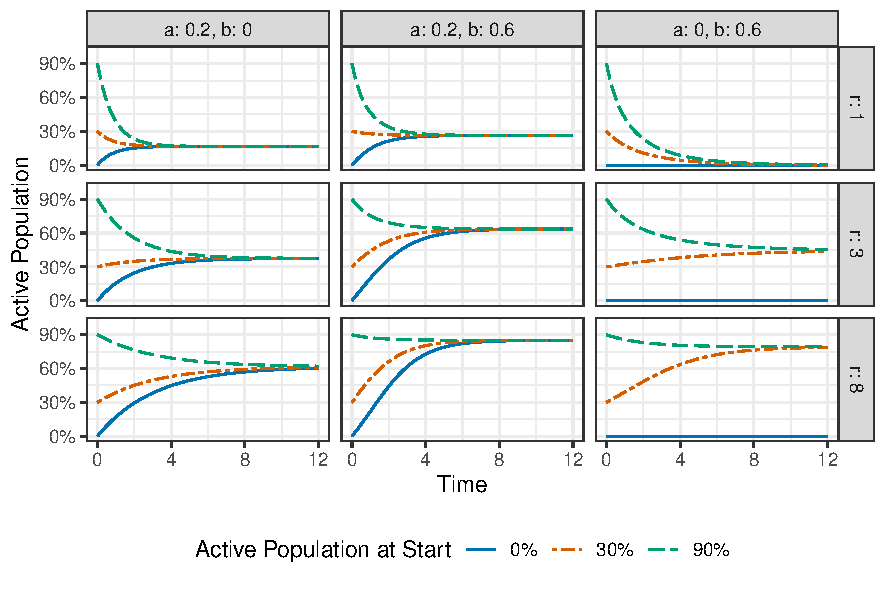
\includegraphics[width=\linewidth]{images/examples_mod_bass.pdf}
\label{fig:examples_mod_bass}
\end{figure}

Figures \ref{fig:examples_mod_bass} and \ref{fig:equi_mod_bass} shall enhance the understanding of the behaviour of the modified models. The former shows example curves of the modified Bass model for selected parameters. The first column represents the special case of the external influence model while the third coumn shows the dynamics with only internal influence. It can be seen that despite the different share of activated population at start, all models converge to the same equilibrium. The only exeption is the blue line in the right column denoting the trajectory of activation in the internal influence model. Without any activations at start, no social activations can ocurr at all. A special case can be found in the top right corner. There, the people forget faster than they can become activated and the diffusion dies, which is the case when $r * b \leq 1$ in internal influence models. Therefore, with an attention span of 1, all rumours, innovations and movements will die out if they are only transmitted socially.

A second observation we can make is that (when the final size is non-zero) the final size of the diffusion is always higher in the row below for the given parameters: The longer the attention span, the more people will be activated in the equilibrium.

\begin{figure}
\caption{The derivative of the modified Bass model for selected parameters}
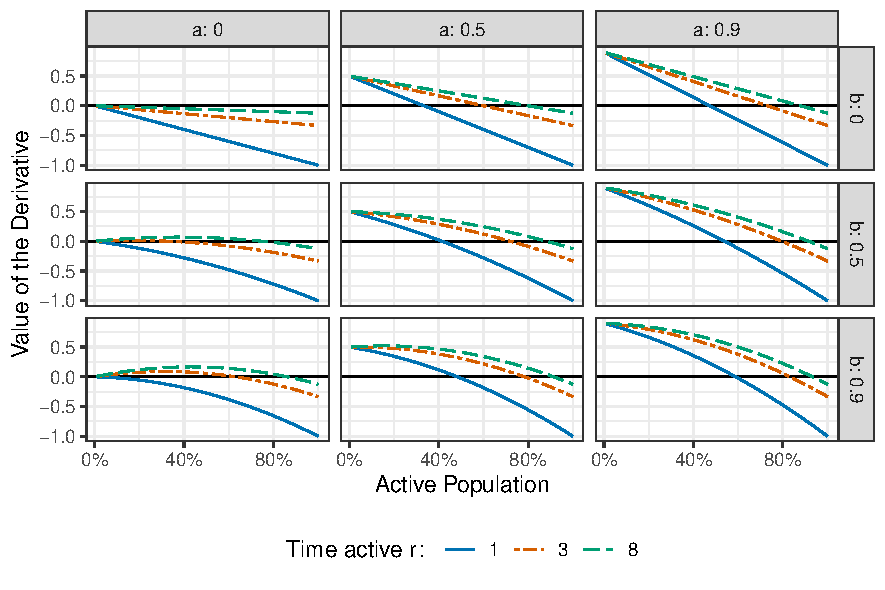
\includegraphics[width=\linewidth]{images/equi_mod_bass.pdf}
\label{fig:equi_mod_bass}
\end{figure}

To better understand the points of equilibria, I included Figure \ref{fig:equi_mod_bass}. It plots the derivative of the modified Bass model for selected values of $a$, $b$ and $r$ including the ones that constitute the special cases of the external and internal influence model over the range of possible states of the activated population. The points where the curves cross the highlighted line $y = 0$ are the equilibria. When the derivative crosses from positive to negative, the equilibrium is stable since a small deviation from the equilibrium results in a dynamic towards the equilibrium again. At points where the drivative crosses from negative positive, a small deviation from the equilibrium is enough to spark a movement away from the unstable equilibrium.

First, the change at no acivated population is determined by $a$ because no social contagions can occur regardless of $b$ and no people can become susceptible again regardless of the attention span $r$ simply because there are none. 

Second, if there is no social contagion, the derivative is linear and the equilibrium is solely determined by the relation of $a$ and $r$. The higher the influence of external sources of activation and the longer the attention span, the higher the equilibrium.
If there is social contagion, $b > 0$, a quadratic term is included and there are two possible solutions for the equilibrium because of the curvature. But these two equilibria are only in the theoretically useful interval if there is no external source. So, in practice there are only two equilibria if the diffusion is purely social, of sufficient size and one of them is definitely 0. But this equilibrium is unstable. When the proportion activated is only slightly over 0, the derivate is positive and the share of activated actors rises. For purely social contagions, 0 can become a stable equilibrium though if people forget faster than can become activated.

Third, we can asess the slope of the diffusion curve in this figure. The positiver the derivate, the faster rises the activated population share and the negativer, the faster does it decline at that point. The impact of external sources $a$ is therefore also extremely important for the overall slope of the diffusion process. But also the internal influence $b$ and the attention span $r$ have a positive impact on the slope. However, since they all converge to different equilibria, they do not necessarily settle earlier.

\section{Network Models}

As beautiful and insightful as mathematical models are, they come with assumptions as discussed before. But there are some particular unrealistic features of the mathematical models that I want to address: they assume that each pair of actors has the same probability of meeting each other, that a simple contact between anyone has the same effectivity of activation and that they assume the population share to be continuous although it is dicreet. And especially unlikely, they are deterministic. 

To tackle these criticisms at least somehow, I use network agent-based modeling to simulate social diffusion in small world networks. While the network structure replaces the assumption of random mixing, using simulations also leads to a certain level of randomness to the process. This randomness might be one reason why not all innovations, informations and movements make it. To explore differences in requirements for activation, I draw upon the distinction of ``simple'' and ``complex'' contagions which I will present first.

\subsection{Simple Contagions in Networks}

The internal influence model can be made more realistic by dropping the assumption of random mixing. Instead, researchers have built computational models simulating diffusion processes in networks. In these models, network structure and the location of the initially infected have a great impact on the diffusion process, especially on the speed of the spread. The shorter average paths lengths in a network, the faster all nodes are infected: the more networks resemble a ``small world'' instead of a ``large world'', the more rapid reaches the process its final size (\cite{wattsCollectiveDynamicsSmallworld1998}). A large world is a network where each node is only connected to its close neighbours while rewiring some of these ties to more distant random others creates ``bridges'' (\cite{granovetterStrenghtWeakTies1973}) between previously distant parts of the network which shorten average path length in these now smaller worlds. The more bridges and therefore the smaller the world, the faster are all nodes infected. The model however tends towards a completely infected population with increasing time like the internal influence model. In some empirical networks or with different network-generating mechanisms it is possible however that there are parts of the network that are not interconnected. Therefore, it is possible that by chance not all nodes get infected.

\subsection{Complex Contagions in Networks}

The theory of complex contagions (\cite[34ff]{centolaHowBehaviorSpreads2018}) combines the network perspective on social diffusion with the threshold model (\cite{granovetterThresholdModelsCollective1978}): a node $i$ is only infected if the threshold $x_{i}$ of infected tie neighbours is reached. How these thresholds are formulated, in absolute or in relative terms, is of consequences though (\cite[50f]{centolaHowBehaviorSpreads2018}). For nodes with few ties, a few infected ties constitute a high share of his network. For a node with many ties, a high relative threshold would require many nodes in the network to be infected in absolute terms. For simplicity, we will work with the absolute formulation of thresholds. However, contrary to the threshold model, the theory of complex contagions shares with the other models that once infected nodes stay infected. This is therefore a generalisation of network contagions because simple contagions can be reformulated as a case where all nodes have an identical threshold of 1: $x_{i} = 1 \ \forall \ i$.

Similarly to simple contagions, network structure has a profound influence on the resulting dynamics. Because nodes need to have at least $x_{i}$ sources of reinforcement, single wide-reaching bridges are not necessarily sufficient to infect distant nodes. If thresholds typically exceed 1, the bridges in small worlds cannot speed up the spread. In the classical formulation of small worlds where some ties are dissolved from a neighbouring node and rewired to a more distant one (\cite{wattsCollectiveDynamicsSmallworld1998}), these bridges actually \textit{slow down} the diffusion process or can even stop contaigon. This is because the infection is held up by bridges that do not have the necessary ``bridge width'' to sustain contagion (\cite[207ff]{centolaHowBehaviorSpreads2018}). The width of a bridge is the number of ties that connect two subnetworks. If the number of ties between an already infected subnetwork and a still susceptible subnetwork is lower than the thresholds of the respective nodes, no infection can take place. Complex contagions therefore spread fastest and most successfully through highly redundant close-knit strong ties.

\subsection{Simulation Setup}

The simulated networks comprise of 100 nodes each and are created using a small world network algorithm where each node is connected to its four immediate neighbours and some random nodes are created with a certain probability. Contrary to the original small world algorithm where where ties are \textit{rewired} (\cite{wattsCollectiveDynamicsSmallworld1998}) and therefore leave gaps in the neighbourhoods of the networks and can therefore stop complex contagions, I \textit{add} the random nodes that also can be between already connected actors (\cite{newmanScalingPercolationSmallworld1999}). The probability of forming a random tie between two networks varies between 0 and 0.18. This results in an increasing number of ties in smaller worlds though as opposed to only changing the structure of the network. I separate the two effects of the number of links and the decreased average path length in regressions. 

I use constant overall thresholds in our models, a threshold of 1 in the simple contagion and a threshold of 2 for a minimally complex contagion. Initially, two connected neighbours are infected. The average attention span can vary between 1 and 10 with smaller steps in between 1 and 3. Longer attention spans have been found to be of little consequence. While a node is always activated when its threshold is met, becoming susceptible again is determined probabilistically and therefore introduces a source of randomness. I consequentially vary only three variables in the simulations: the activation threshold, the probability for added random ties and the average attention span.

The network models are programmed in \textit{NetLogo} (\cite{wilenskyNetLogo1999}\nocite{wilenskyNetLogoSmallWorlds2005}). The individual models end after 75 ticks. The data from the agent-based model and the depictions of the mathematical models are done in \textit{R 3.6.3} (\cite{rcoreteamLanguageEnvironmentStatistical2020}\nocite{wickhamGgplot2ElegantGraphics2009}). Constructed variables of interest include the mean number of activated nodes and the standard deviation of each single simulation run in the last third of the run time. At this time, most runs settled around their equilibrium or deceased. Also a dummy was created whether the run ended with no activated population. To assess the average slope of the diffusion curve, I divided the mean number of activated nodes in the last third by the time it took to cross above this value first from the start. All code and the simulated data used for this article can be retrieved from the \href{https://osf.io/ykhdv/}{project page at the Open Science Framework}.

\subsection{Results}

\begin{figure}
\caption{Examples}
\centering
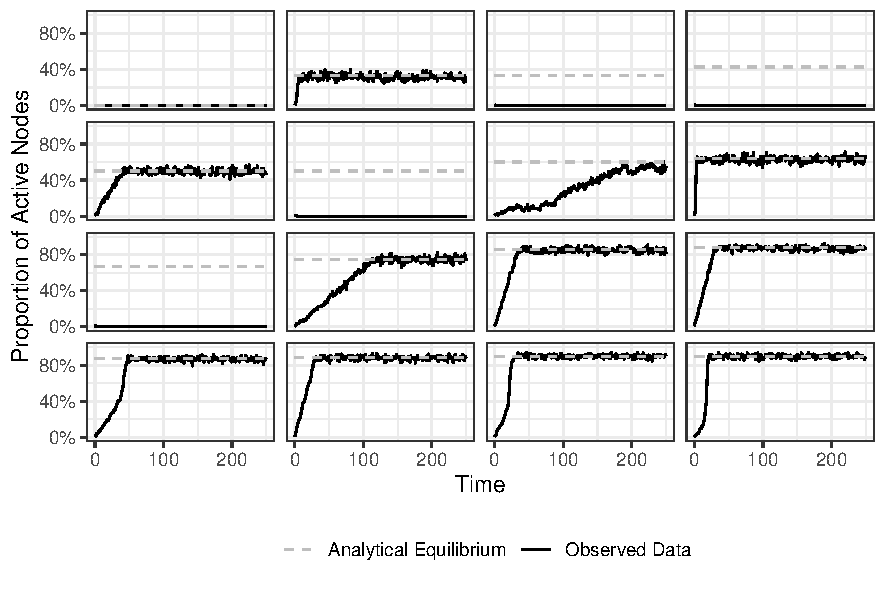
\includegraphics[width=\linewidth]{images/example_runs.pdf}
\label{fig:examples}
\end{figure}

To provide a first understanding, Figure \ref{fig:examples} shows some exemplary single trajectories. There are two possible final states visible here: either the diffusion ends with no one activated (since this is a purely social diffusion, once the process is at 0 it cannot change anymore) or the process fluctuates around the analytical solution obtained from the equivalent mathematical model. However, for the process to die, the number of activated nodes needs to be low of course. This happens typically early on but when the slope of the curve is lower, this can still happen later on. In run 4562, the process rises at first and then dies while in the other examples where the process dies it happens even earlier. In run 86, no activated population is actually the equilibrium. Since nodes are always activated if their threshold is reached ($b = 1$), this is reached only by an attention span $r = 1$. 

We also observe that the slopes until the final size is reached vary considerably even if the final states are similar. While we can already can suspect that simple contagions are faster, especially the smaller the world is, I will show this in further detail in a moment.

\begin{figure}
\caption{Deviation from the analytical Equilibrium and Probability of Dying}
\begin{subfigure}{.5\textwidth}
\centering
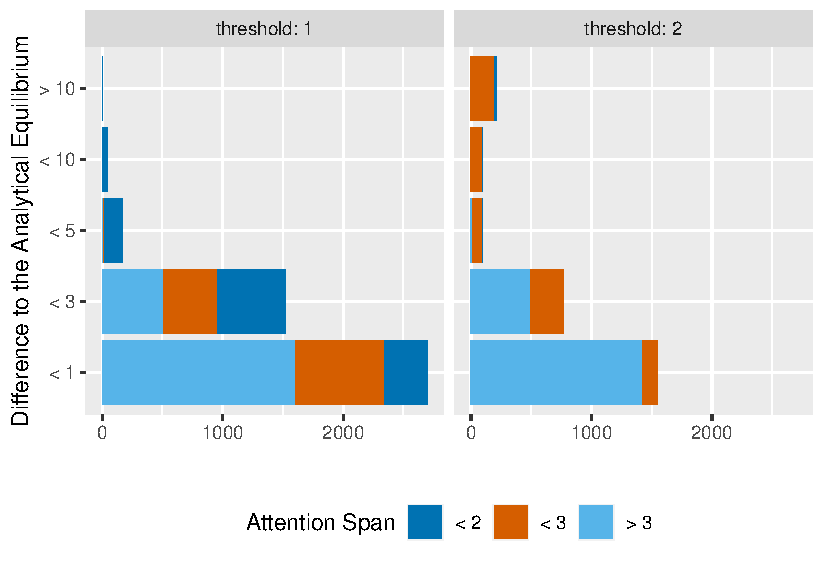
\includegraphics[width=\linewidth]{images/difference.pdf}
\caption{Absolute Difference}
\end{subfigure}
\begin{subfigure}{.5\textwidth}
\centering
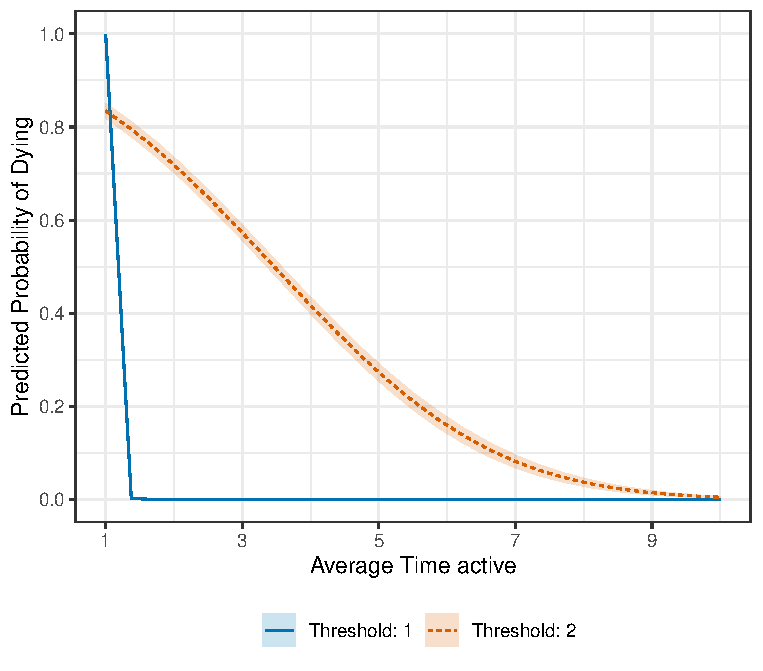
\includegraphics[width=\linewidth]{images/died_attention_span.pdf}
\caption{Predicted Probability with 95\% CIs}
\end{subfigure}
\label{fig:dev_die}
\end{figure}

The impression that the trajectories match quite close the analytical equilibrium if they do not die before is further supported by Figure \ref{fig:dev_die}a. The average number of activated nodes in the last third of the observed timespan deviates from the analytical equilibrium only by an absolute difference of below three percentage points for most observations. This holds for both thresholds. But there are fewer observations with a small deviation from the equilibrium for the complex contagions. This is partly due to that more complex contagions have died. This can be seen in that image already because almost no observations from the category of an attention span of below two are present. But there are also more observations with higher deviations in the case of complex contagions. They are mostly from the category of an attention span between two and three. I will come back to this finding. For observations with longer attention spans, deviations are overwhelmingly small regardless of threshold.

Probably the most remarkable finding of the agent-based model is that the probability of the diffusion process dying from the randomness in the fluctuations is extrordinarily higher for complex contagions. Figure \ref{fig:dev_die}b shows the predicted probabilities of dying by attention span at the means of the network variables from separate probit regressions for the two thresholds. The observations with an attention span of one are excluded because their equilibrium is at zero. But whereas the probability of dying is marginal even at an attention span of slightly larger than 1 for simple contagions, complex contagions have a considerable probability of ending with no activated population over a wide range of attention spans. But the expectable negative relation between attention span and the probability of dying is prominent.

\begin{figure}
\caption{Slopes until the Equilibrium}
\begin{subfigure}{.5\textwidth}
\centering
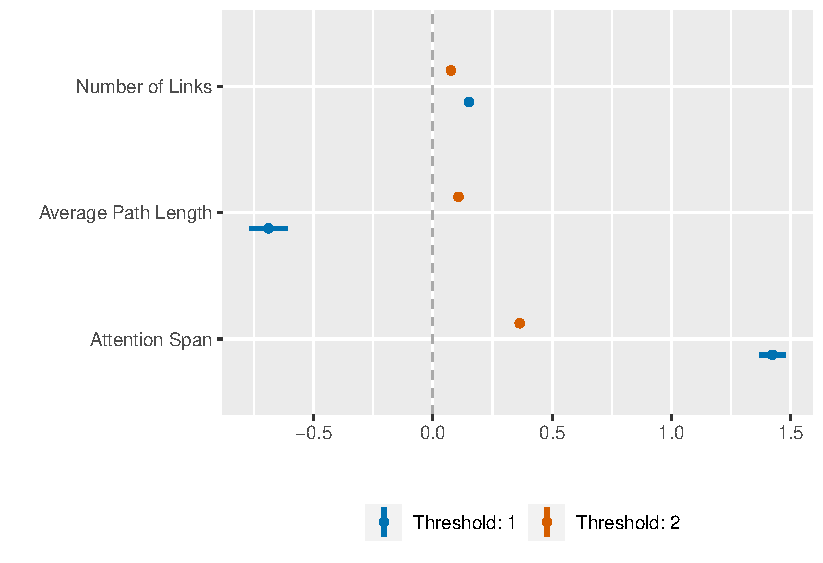
\includegraphics[width=\linewidth]{images/slopes_coef.pdf}
\caption{OLS coefficients with 95\% CIs}
\end{subfigure}
\begin{subfigure}{.5\textwidth}
\centering
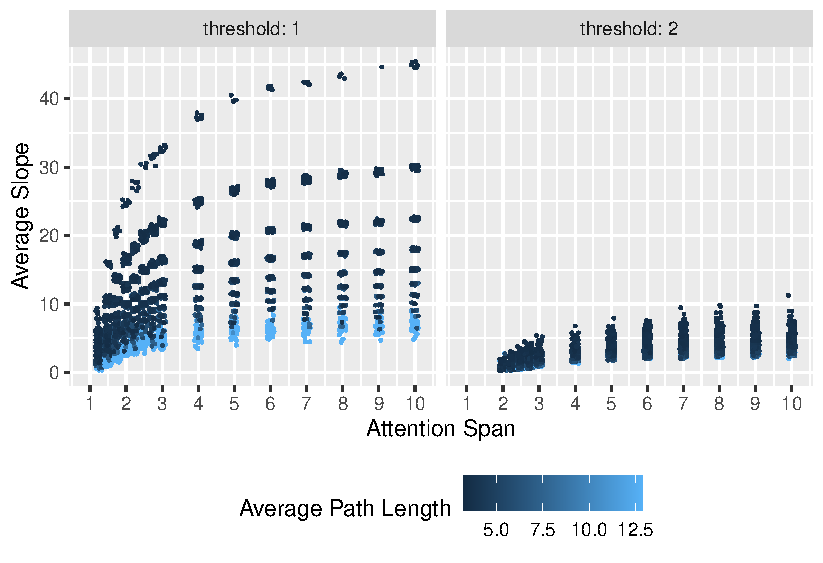
\includegraphics[width=\linewidth]{images/slopes_scatter.pdf}
\caption{Scatter Plot}
\end{subfigure}
\label{fig:slope}
\end{figure}

When assessing the average slope of the diffusion curve until they first surpass their average in the last third in Figure \ref{fig:slope}a, we can see that the average path length has a strong negative effect on the average slope of simple contagions: the lower the average path length, the faster does a simple contagion reach its final size. For complex contagions, however, the effect is even slightly positive for whatever reason. Unsurprisingly, a higher number of ties has a slight positive effect for both but it is more pronounced for simple contagions again. Complex contagions do benefit from more ties though because it increases the chance that a node has two already activated neighbours.

The effect of attention span on the average slope is the largest in magnitude for both types of contagions. The longer the attention span, the higher is the slope. Like in the mathematical models, we can separate two processes: the susceptibles becoming activated and the activated becoming susceptible. The latter is determined by the attention span. With a longer attention span, fewer nodes become susceptible again per time unit. This means that more nodes are still able to activate others and they do not need to be reactivated.

I suspect both the higher probability of dying over a wider range of attention spans and the higher number of observations with high deviations from the analytical equilibrium in the last third of the observation window to be linked to a crucial difference between simple and complex contagions: their speed of spread. Not only the effects of the different variables varies by threshold but they differ remarkably in their overall levels as shown in Figure \ref{fig:slope}b. In the original large world where every node is connected to its four immediate neighbours, simple contagions are double as fast as complex contagions: while the two initially activated nodes can activate their two neighbours to the left and their two neighbours to the right in the simple contagion, in the complex contagion, they can only activate one at each side. When random ties are added, more nodes can get activated in a single time step that can span over to distant parts of the networks in simple contagions. This dramatically increases the spreading speed because one activated node in a largely unactivated network can activate its four neighbours and not only the two to one side like when the other side is already activated. For complex contagions, these additional random ties are of far less consequence: a single tie is not sufficient to activate a distanced node and an isolated distant node cannot activate further others. This means that a complex contagion still spreads mainly through the short ties from neighbour to neighbour. Only if a random tie connects a susceptible node to an activated one, this one will become activated faster if its neighbours become activated. In short, complex contagions are much slower than simple contagions to begin with and barely profit from the changes in network structure as well.

These differences in speed causes complex contagions to remain longer in the ``danger zone'' where they might hit zero activated nodes from a random fluctuation and die. And because their speed is relatively slow even at longer attention spans, this still holds for longer compared to simple contagions. Simple contagions gain a lot of speed when the probability of becoming susceptible again is lower. Therefore, they reach their ``critical mass'' faster. 

Complex contagions being slow also affects the deviations from the analytical equilibrium in the last third of the observation time presented in Figure \ref{fig:dev_die}: the chosen operationalisation of averaging the number of activated nodes in the last third of the 75 steps is too early for them. While most others have long settled around their equilibrium at that point, they are so slow that they have not reached it yet. The observation that complex contagions differ more from the analytical equilibrium is therefore caused by a methodological choice. The diffusion process still either dies or matches the mathematical prediction quite close in the end.

\begin{figure}
\caption{Fluctuations around the Equilibrium}
\begin{subfigure}{.5\textwidth}
\centering
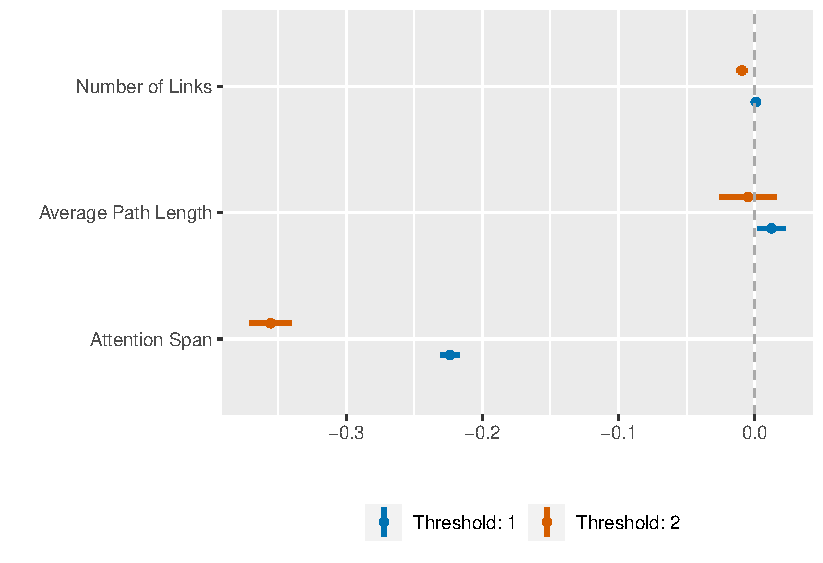
\includegraphics[width=\linewidth]{images/sd_coef.pdf}
\caption{OLS coefficients with 95\% CIs}
\end{subfigure}
\begin{subfigure}{.5\textwidth}
\centering
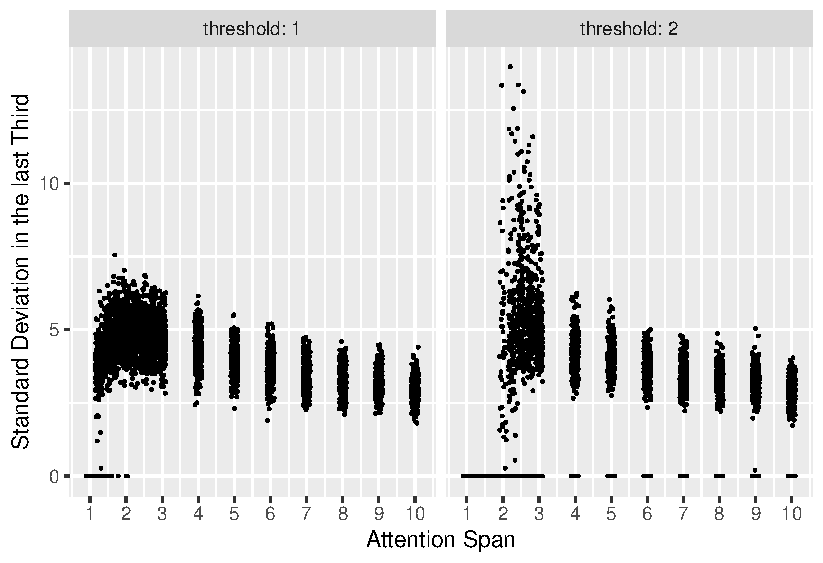
\includegraphics[width=\linewidth]{images/sd_scatter.pdf}
\caption{Scatter Plot}
\end{subfigure}
\label{fig:sd}
\end{figure}

The last property I examine is how strong the fluctuation around the equilibrium is. Figure \ref{fig:sd} shows the results. Network characteristics have no or extremely small effects. We could have expected that with more ties, the chance of getting reinfected rises. But the effect of the additional ties is nonexistent for simple contagions. The existing ones are sufficient to reactivate the nodes. The effect is existent for complex contagions though. Because two ties with activated nodes are needed to get reactivated, additional ties increase the probability of having two activated nodes in the ego network. But the effect is marginal. There is a significant decrease in the standard deviation in the last third of the observation window by attention span though. The final state is more stable with higher attention spans because fewer nodes become susceptible again at each time step. 

That the effect of attention span is more prominent for complex contagions is caused by the outliers for very low attention spans observable in subfigure \ref{fig:sd}b. This is again the methodological problem that these observations have not reached their equilibrium yet. They are still on the upwards trend and therefore have a higher variation in the last third of the observation window. The low outliers are potentially observations that were still living at the beginning of the last third but died eventually. Their standard deviation is so low because they have no variation after a while anymore. The observations with a standard deviation of zero have died before. We can see again that complex contagions die even with higher attention spans. But overall, the amount of fluctuations in the last third of time is very comparable between simple and complex contagions if they reach their equilibrium.

\section{Discussion}

In this article, I have shown how the average time an actor remains activated can change the dynamics of diffusion processes. We can think of this time as the average attention span an actor has for a piece of information, a rumour, a social cause or collective action. Attention span has both an impact on speed and the final size of a diffusion: The longer the attention span, the steeper the gains until the equilibrium and the more people will be finally activated. My modification of the Bass model even isolates conditions where a mathematical model predicts a diffusion process to fail entirely and therefore overcomes major shortcomings of the previous models which predict every diffusion process to spread to the whole initially susceptible population eventually. My modified mathematical models show that in purely social diffusion processes, no activated population is always an equilibrium and can become the only one if the attention span is too short and the effectiveness of contact is too low so that the losses exceed the gains.

But arguably, mathematical models have limitations that hold true for my modified models as well. First, they assume an equal probability of getting activated for all and in the case of social diffusions they still assume random mixing which means that the probability of meeting someone to activate them is constant as well. Second, the proportion of the population that is activated is assumed to be a continuous variable although bound between zero and one hundred percent. In reality, the number of activated people is discreet. How well the approximation as continous works depends on the size of the population. And third, mathematical models are deterministic although there is a certain randomness to the world.

I at least started to address these three shortcomings by implementing the ideas of the mathematical models in a network agent-based model of a socially driven diffusion process. The assumption of random mixing is exchanged for a close-knit community structure with a specified probability of added random ties and the continous perspective of the population is exchanged for a fixed constant population of 100 nodes. Although I still assume the same conditions for every actor to get activated, I vary it between runs to distinguish between simple and complex contagions (\cite{centolaHowBehaviorSpreads2018}). 

And indeed, there are remarkable differences between the two types of models and the two types of conditions for activation. While the overall relations between attention span and spreading behaviour from the mathematical models hold and the small world network structure has the expected effects on spreading speed, the inherent randomness of the model is an important explanation why complex contagions fail so frequently. Because complex contagions spread so slow and cannot benefit from bridging ties, they require more time to reach the critical mass of activated nodes that prevents them from dying out by random fluctuations. Therefore, the overall probability of failing is much higher and even persists at long attention spans. This is therefore another contribution to the initial question of Damon Centola why some types of contagions do not make it: when the spreading speed is too slow, some simple randomness is enough to end a diffusion. Reversability and attention span potentially are crucially linked to the speed, size and chances of success of social phenomena that are associated with higher costs or more uncertainty.

But neither do these agent-based models resolve all issues regarding the mathematical models, nor are they free of assumptions. They are still based on a binary conception of activation and assume constant parameters and population throughout for example. But it might be more realistic to assume that the activation consists of several steps. In these different stages, the ability to activate others may also vary. Or actors activate others only for a limited time as long as they think it is new enough to talk about and external sources like advertising campaigns might end. The respective conditions and availability to get activate can not only vary over time but between individuals. But creating agent-based models involves typically a trade-off between realism on one hand and simplicity and therefore understandability on the other. For the most part, the theoretical advances achieved from an agent-based model are most clear and pronounced when the model is simple  (\cite{flacheSocialDynamicsBottom2011}). For a(n older) review of models that try to overcome some of these shortcomings in the field of product diffusion, see Mahajan et al. (\citeyear{mahajanNewProductDiffusion1990}). 

The way how I incorporated attention span has an underlying assumption as well. In the mathematical models, it works deterministically again: a constant proportion switches from activated to susceptible. In the agent-based models, this works probabilistically but that typically results in a normally distributed variable. If attention span is not normally distributed among actors, this might be of consequence for the behaviour. If some actors have an exceptionally long attention span for example, the probability of dying out from random fluctuations is reduced even though the mean is the same. This limitation could require sensitivity checks in the future. Similarly, I used only one type of network structure. Although diffusion processes in different networks are quite well understood, potential interactions between attention span and a wider range of network structures have not been studied by me.

In summary, I think that dropping the assumption of irreversability in diffusion models and to incorporate the time an actor is on average activated has shown to be of rather drastic consequences in speed, final size and probability of surviving. Especially for diffusion processes sociologists are often interested in like the spread of information and behaviour, this might be a fruitful way of conceptualising their spread. Whether the addition of a third parameter to the Bass model improves our understanding of real-life diffusion processes in a way that is worth the extra parameter, remains to be answered empirically.


\printbibliography

\section*{Mathematical Appendix}

\subsection*{Equilibria of the modified Bass Model}

The equilibrium needs to fulfill the condition $\frac{\delta p_{act}(t)}{\delta t} = 0$. 

$a \in [0;1] \ \land \ b \ \in \ ]0;1] \ \land \ r > 1$.

\begin{align*}
& \frac{\delta p_{act}(t)}{\delta t} = a (1 - p_{act}(t)) + b \ p_{act}(t) \ (1 - p_{act}(t))  - \frac{1}{r} \ p_{act}(t) \\
&\implies 0 = a (1 - p_{act}^{*}) + b \ p_{act}^{*} \ (1 - p_{act}^{*})  - \frac{1}{r} \ p_{act}^{*} \\
&\iff 0 = - b \ p_{act}^{*2} - (a - b + \frac{1}{r}) \ p_{act}^{*} + a \\
&\iff 0 = p_{act}^{*2} + \frac{a - b + \frac{1}{r}}{b} \ p_{act}^{*} - \frac{a}{b} \\
\end{align*}

applying the p-q-formula

\begin{align*}
&\implies p_{act}^{*} = - \frac{a - b + \frac{1}{r}}{2b} \pm \sqrt{\left( \frac{a - b + \frac{1}{r}}{2b} \right)^2 + \frac{a}{b}} \\
\end{align*}

for $a = 0 \ \land \ b \ \in \ ]0;1] \ \land \ r > 1$ (solution for the internal influence model).

\begin{align*}
&\implies p_{act}^{*} = - \frac{- b + \frac{1}{r}}{2b} \pm \sqrt{\left( \frac{- b + \frac{1}{r}}{2b} \right)^2 } \\
&\iff p_{act}^{*} = - \frac{- b + \frac{1}{r}}{2b} \pm \frac{- b + \frac{1}{r}}{2b} \\
&\iff p_{act}^{*} = 0 \ \land \  - \frac{- b + \frac{1}{r}}{2b} - \frac{- b + \frac{1}{r}}{2b} \\
&\iff p_{act}^{*} = 0 \ \land \  \frac{b - \frac{1}{r}}{b} \\
&\iff p_{act}^{*} = 0 \ \land 1 - \frac{1}{rb} \\
\end{align*}

for $a  \ \in \ ]0;1] \ \land \ b \ \in \ ]0;1] \ \land \ r > 1$.

\begin{align*}
&\implies  - \frac{a - b + \frac{1}{r}}{2b} - \sqrt{\left( \frac{a - b + \frac{1}{r}}{2b} \right)^2 - \frac{a}{b}} < 0 \\
&\implies  - \frac{a - b + \frac{1}{r}}{2b} + \sqrt{\left( \frac{a - b + \frac{1}{r}}{2b} \right)^2 - \frac{a}{b}} > 0 \\
\end{align*}

Because $p_{act}^{*}$ constitutes a population share it is restricted to be part of the interval [0;1]. One of the two possible analytical solutions in this case is definitively negative however and therefore theoretically not possible. Therefore, there is only one equilibrium in this case:
    
\begin{align*}
&p_{act}^{*} = - \frac{a - b + \frac{1}{r}}{2b} + \sqrt{\left( \frac{a - b + \frac{1}{r}}{2b} \right)^2 + \frac{a}{b}} \\
\end{align*}


\subsection*{Equilibrium of the modified External Influence Model}

The external influence model is the special case of the Bass model with $b = 0$. But because dividing by 0 is not defined, we cannot derive the equilibrium from the p-q-formula of the general model above. Starting point is therefore the original differential equation of the external influence model. The equilibrium needs to fulfill the condition $\frac{\delta p_{act}(t)}{\delta t} = 0$.

\begin{align*}
 & \frac{\delta p_{act}(t)}{\delta t} = a \ (1 - p_{act}(t)) - \frac{1}{r} \ p_{act}(t) \\
&\implies 0 = a \ (1 - p_{act}^{*}) - \frac{1}{r} \ p_{act}^{*} \\
&\iff \frac{1}{r} \ p_{act}^{*} = a - a  \ p_{act}^{*} \\
&\iff  (a + \frac{1}{r}) \ p_{act}^{*} = a \\
&\iff p_{act}^{*} = \frac{a}{a + \frac{1}{r}}
\end{align*}

\end{document}
